
\section{Detector Operations}
During the third quarter, the LHC restarted operations and the CMS experiment and after a commissioning period began taking physics quality data. Much of the earliest running has been dedicated to the commissioning of new elements of the detector that have be installed during the  year end technical stop.   Most significant of these upgrades was the completely new pixel system.   The metrics reported for the various subsystems exclude commissioning periods but rather only refer to physics operations.  As shown in figure~\ref{fig:Lumi} an impressive 5.33 fb$^-1$ was recorded by CMS during this period.


\begin{figure}
\begin{center}
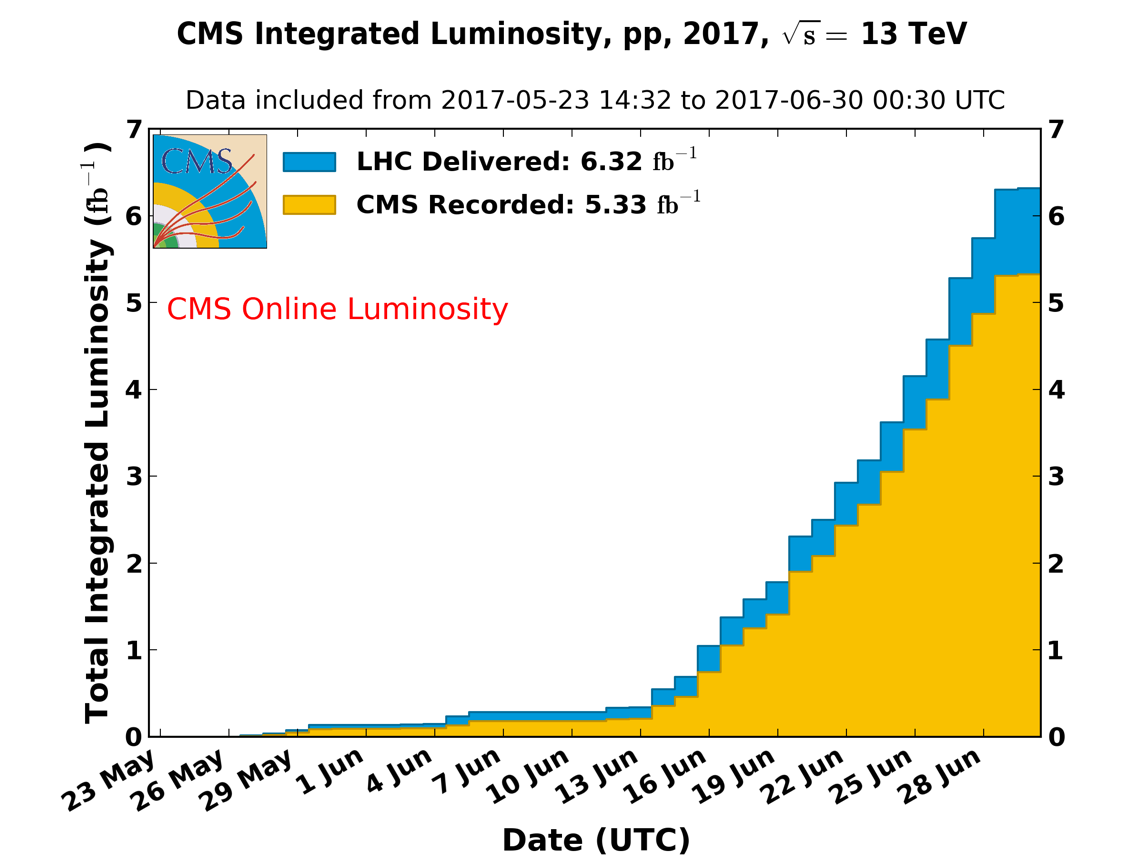
\includegraphics[width=0.66\textwidth]{Picture1.png}
\caption{Luminosity, delivered by the LHC and recorded by CMS, through June 30.}
\label{fig:Lumi}
\end{center}
\end{figure}

\subsection{BRIL }
The Pixel Luminosity Telescope (PLT) together with the fast beam condition monitor (BCM1F) and HF are operational and provided online luminosity measurements since first beams arrived. The PLT has been aligned and the repaired telescopes are functional. The fast readout for all telescopes works but two telescopes exhibit degraded full pixel information that is used for track-based studies. The latter also provided a fast measurement of the beam spot and allows tracking of beam conditions. Publication of luminosity and beam background measurements is continuous. For the calibration of the luminosity a first high-luminosity VdM scan was performed and for the online luminosity now regularly information from a short beam-scan at the beginning and end of the fill is used. Corrections for efficiency and accidentals are obtained with fast turnaround after completion of a fill. Systematic beam studies with LHC were performed and the procedures are setup for the full VdM scan program this month. 

The PLT detector is scheduled for replacement in 2019 due to the expected radiation damage. As the detectors use analog readout old parts have to be secured. Critical is the availability of port cards and slow-hub chips for four opto-motherboards – only 4 are left. A design modification for an alternative chip is explored. A test stand for component testing is in preparation at Rutgers and CERN.

\begin{table}[htp]
\caption{BRIL Metrics}
\begin{center}
\begin{tabular}{|l|r|}
\hline
Working Metric&Performance\\
\hline
Fraction of telescopes fully operational &  90\% \\
\hline
Efficiency of delivery of lumi histograms &  $>$ 99\% \\
\hline
Uptime of lumi  histogram production & $>$ 99\% \\
\hline
Lumi lost & 0 /pb \\
\hline
\end{tabular}
\end{center}
\label{BRILMetrics}
\end{table}%


\begin{table}[htp]
\caption{BRIL Milestones}
\begin{center}
\begin{tabular}{|l|l|r|r|}
\hline
Subsystem&Description&Scheduled&Achieved\\
\hline
BRIL & Update Lumi for 2016
& March 1& March 1\\
\hline
BRIL& Ready for Physics & May 1& May 1   \\
\hline
BRIL & Improve 2017 Lumi numbers & Dec 1 &  \\
\hline
\end{tabular}
\end{center}
\label{BRILMIlestones}
\end{table}%



\subsection{Tracker }

The tracker is able to reconstruct good quality tracks and it looks like the performance is as good as the Phase 0 tracker (see below). There are issues,  however, with the Barrel Pixel layer 1 detector efficiency and a separate issue with the Token Bit Manager chip freezing up during collisions. These two issues currently limit us from pronouncing the whole Pixel detector ready for physics.

\subsubsection{Pixels }

Soon after stable beam collisions started, it was discovered during timing scans that the BPiX layer 1 and layer 2, which share a common fine delay setting, could not both be timed in to a common optimal operating point. Instead, a compromise point, at the timing plateau end for layer 2 and beginning for layer 1, was chosen until the timing can be adjusted in hardware at a time when the BPiX can be removed for adjustment. There also appears to be an efficiency loss in the layer 1 chip, yet to be understood, leading to single hit clusters being reconstructed as two clusters (aka ``broken hit clusters"). Further, it was determined that the modules closest to the beam in the layer 1 BPiX are already operating at the maximum design luminosity. We are exploring different settings for layer 1 chip operating constants and different timing strategies to try and optimize physics performance. As a reminder, BPIX layers 2-4 and FPIX utilize the PSI46dig readout chip everywhere, while BPIX layer 1 uses the PROC600 chip.  The PSI46dig is a minor upgrade to the Phase 0 chip, while the PROC600 is an entirely new chip designed to withstand the fluences expected in layer 1.

There is also an issue with all versions of the Token Bit Manager (TBM) chip. Two TBM cores are present in each module.  About 20 detector channels (out of ~5,000) per hour stop responding to triggers and are only recoverable with a local power cycle of the module containing the TBM. The TBMs closest to the beam are affected the most, and the effect is the same as a Single Event Upset on a vulnerable flip flop in the design. We currently perform the local power cycle when about 4\% of the layer 1 channels are not responding. The recovery operation is manual and adds about 5\% deadtime to operations. We are adding software and firmware to speed up and increase the automation of the recovery time.

In the metrics it is to be noted that there is an additional 418/pb of luminosity used to investigate the issues with the Phase 1 pixel detector. CMS does not count this as pixel deadtime but adds it to the ``General" category of lost luminosity along with tests and such from
other detectors (an additional 60/pb).

\subsubsection{Strips}

The strip detector primary beam on calibrations were completed soon after stable beam collisions started and the strip detector appears to be operating well in 2017 collisions. Some detailed studies of efficiency and performance need the pixels in a stable data taking condition, though there does not appear any cause for concern in the performance of the strips.

\vskip 0.2in

\begin{table}[htp]
\caption{Tracker Metrics}
\begin{center}
\begin{tabular}{|l|c|c|}
\hline
 &Pixels&Strips\\
\hline
\% Working channels & 95.6 &  96.2 \\
\hline
Downtime attributed in pb$^{-1}$& 48.44 & 25.24 \\
Fraction of downtime attributed (\%)& 6.3 & 3.3\\
\hline
\end{tabular}
\end{center}
\label{TrackerMetrics}
\end{table}%


\begin{table}[htp]
\caption{Tracker Milestones}
\begin{center}
\begin{tabular}{|l|l|r|r|}
\hline
Subsystem&Description&Scheduled&Achieved\\
\hline
Tracker & Pixel Phase 0 Detector Removed&Feb 15&Jan 23 \\
\hline
Tracker & Pixel Phase 1 Detector Installed &Mar 30 &Mar 12 \\
\hline
Tracker & Pixel Phase 1 Detector & & \\ 
        & Ready for Collisions  &May 5 & \\
\hline
\end{tabular}
\end{center}
\label{TrackerMilestones}
\end{table}%



\subsection{ECAL }
The second quarter was devoted to the preparations for running. The detector was bought into fully operational status in the first quarter. In the second quarter no major problems with the detector have been encountered. The standard set of procedures for preparing for the run were conducted.  These include a series of cosmic runs to debug the various DAQ/Trigger/monitoring issues that normally arise. New pedestals, pulse shapes, timing constants, laser monitoring corrections and selective readout thresholds have been installed. At the present time we are running with 2016 energy calibration constants. This is because the new constants are derived from data and it takes several weeks to generate the initial values after data taking has begun. The 2016 constants provide a fairly good starting point. The early data looks as expected and plots of the pizero and Z boson mass were approved to be shown at the major conferences. 



\vskip 0.2in


\begin{table}[htp]
\caption{ECAL Metrics}
\begin{center}
\begin{tabular}{|l|r|}
\hline
Metric&Performance\\
\hline
Fraction of channels operational: EB& 99\% \\
\hline
Fraction of channels operational: EE& 98.4\%\\
\hline
Fraction of channels operational: ES& 99.9\%\\
\hline
Downtime attributed pb$^{-1}$ & 15.2 \\
Fraction of downtime attributed& 2\% \\
\hline
Resolution performance & 2.5\% \\
\hline
\end{tabular}
\end{center}
\label{ECALMetrics}
\end{table}%


\begin{table}[htp]
\caption{ECAL Milestones}
\begin{center}
\begin{tabular}{|l|l|r|r|}
\hline
Subsystem&Description&Scheduled&Achieved\\
\hline
ECAL & Refurbish Maraton to provide& &\\
     & redundant thermal interlock &March 1& March1 \\
\hline
ECAL & Replace Laser Diode & March 1& March 1\\
\hline
ECAL & Ready for Beam& May 1& May  1 \\
\hline
ECAL & Preliminary Calibration& June 15& July 15 \\
\hline
\end{tabular}
\end{center}
\label{ECALMilestones}
\end{table}%



\subsection{HCAL}




During the second quarter of 2017, the HCAL Operations group focused on commissioning
the HF and partial HE Phase I upgrades, and then on calibrating the HCAL and on taking data.

\vspace*{2mm}

For HF, the upgrade consists of installing
dual-anode readout. New 
front-end electronics was also installed to support increased number of channels.
The old QIE8s (7bit ADC) were replaced with QIE10s (8bit ADC).
The new front-end electronics also has an embedded TDC which will be used to discriminate 
physics signals from showers in the 
HF calorimeter from spurious signals due to Cerenkov light from particles directly hitting the photo-tube windows.

All the components for the HF upgrades were installed ahead of schedule by mid-March, and the detector was 
ready for physics by May 1. First calibrations have been completed and timing has been equalized for all channels.
There are currently two issues with the HF. First, the HF low voltage (LV) power supplies are experiencing a
high rate of single event upsets (SEUs) when the beam is on leading to a small amount of deadtime.
The problem has been traced to prototype LV supplies which have a factor of 20 higher rate of SEUs than
the production supplies. The power supplies will be re-arranged during the Technical Stop in early July
so that production supplies will provide all the HF LV. Second, there is noise at HF IETA = -30 and -29.
It has been determined that this noise was also present in the 2016 data, but the cause is still unclear.

\vspace*{2mm}

For HE, one upgraded HE readout box (out of 36) was installed
to obtain experience with upgraded system. The upgraded HE readout box (HEP17)
is performing well. The gains and pulse shapes from HEP17 have now been adjusted in the reconstruction
to match what is observed in the data. (A similar small HF upgrade installation was done
last year, and the experience gained with the upgraded system informed this year's HF EYETS work.)

\vspace*{2mm}

First calibrations for HF, HB, HE, and HO have been obtained. 

\vspace*{2mm}

Planning to install the complete HE upgrade in 2017-18 YETS is in progress, and a draft detailed schedule
including personnel needs has been completed, and is being optimized. 

\vspace*{3mm}

\noindent {\it Metrics and Milestones for this Quarter} \\

\noindent June 1 Milestones \\
HF Detector Commissioned. This milestone was achieved May 1. \\
HCAL Ready for Physics. This milestone was achieved May 15.



\vskip 0.2in


\begin{table}[htp]
\caption{HCAL Metrics}
\begin{center}
\begin{tabular}{|l|r|}
\hline
Metric&Performance\\
\hline
Fraction of channels operational: HF& 100\%\ \\
\hline
Fraction of channels operational: HE& 99.63\%\ \\
\hline
Fraction of channels operational: HB& 99.77\% \\
\hline
Fraction of channels operational: HO& 99.72\%  \\
\hline
Downtime attributed pb$^{-1}$ & 16.3 \\
Fraction of downtime attributed& 1.69\%\ \\
\hline
Abs Energy Calibration & 5\% \\
\hline
Inter-calibration Uniformity & 5\% \\
\hline
\end{tabular}
\end{center}
\label{HCALMetrics}
\end{table}%


\begin{table}[htp]
\caption{HCAL Milestones}
\begin{center}
\begin{tabular}{|l|l|r|r|}
\hline
Subsystem&Description&Scheduled&Achieved\\
\hline
HCAL& HF Phase 1 Installed & April 1 &  March 15 \\
\hline
HCAL& HF Detector Commissioned & June 1 & May 1\\
\hline
HCAL& Ready for Physics & June 1 & May 15\\
\hline
\end{tabular}
\end{center}
\label{HCALMilestones}
\end{table}%








\subsection{EMU }


After the detector was closed and the CMS solenoid field was ramped up, water was 
detected accumulating at the bottom of the detector.  After a lengthy processes,
the source was localized to a leak in one of the ME1/1 cooling circuits on the YE-1 endcap disk.
That circuit was shut off to stop the leak, but this left two chambers 
(ME-1/1/34 and ME-1/1/35) without cooling, so they remain powered down and disabled.
The first opportunity to investigate the leak in more detail should come at 
the year-end technical stop.  

Two other chambers (ME-2/1/3 and ME-4/2/21) are disabled due to low voltage problems. Both have shown  similar problem before, but the low voltage connections on these chambers are difficult to access.  They will be investigated further during the first technical stop in July.

In total, the CSC system finishes the quarter with four out of 540 chambers disabled.

Otherwise, the CSC system operated smoothly in the LHC start up and is performing
efficiently in global data taking. Occasional problems with corrupt data are being 
reported by the FED system.  These are being investigated, but they do not contribute
 significant downtime (<0.5\%). Some HV instabilities were detected in the high-eta chambers (ME1/1) caused by fast ramping of the luminosity which might lead to Malter currents in some planes. We are recovering from those by lowering slightly the HV and by performing reverse polarity training during the technical stop.

Some of the early collision runs were used to refine the timing constants for the 
ME1/1 chambers.  The timing on these chambers had shifted slightly in the Fall of
 2016 due to a correction in the strip comparator threshold settings.

The 5 new GE1/1 demonstrator chambers were installed adjacent to the CSC chambers,
and investigations were carried out to understand under what conditions the GE1/1
system induced noise in the CSCs.  The parts that induced noise were disabled for
 the time being. 

Data collected on June 14 with a dedicated single-layer trigger were used to study the induced background hit rates. After modifications to the shielding in the forward rotating shielding, done during EYETS, the recorded levels look rather similar to 2016 except for an improved uniformity between -z and +z detector ends and a somewhat lower background rate (~20-30\%) in the outer rings of the CSC system.


\vskip 0.2in

\begin{table}[htp]
\caption{CSC Metrics}
\begin{center}
\begin{tabular}{|l|c|}
\hline
 \% Working channels & 98.4\%  \\
\hline
Downtime attributed pb$^{-1}$ & 1.5 \\
Fraction of downtime attributed& 0.2\% \\
\hline
Median spatial resolution &  126 $\mu$m \\
\hline
\end{tabular}
\end{center}
\label{CSCMetrics}
\end{table}%



 \begin{table}[htp]
\caption{EMU Milestones}
\begin{center}
\begin{tabular}{|l|l|r|r|}
\hline
Subsystem&Description&Scheduled&Achieved\\
EMU& CSC ready for physics& May 1& April 29 \\
\hline
EMU& Firmware to mitigate & &\\ 
   & DCFEB EPROM problem &July 1 & January 29 \\
\hline
EMU & New HV settings for  & & \\
&reduced gain & August 1 &  \\
\hline
\end{tabular}
\end{center}
\label{EMUMilestones}
\end{table}%


\subsection{DAQ}
The DAQ group finished the commissioning of the readout links for the subsystems which are new or have been upgraded during EYETS. New readout links were installed for GEM. 
Functionality has been added to support multiple DAQ links from the same HCAL backend card, while using a single TCDS link. This was required to accommodate larger fragment sizes in 2017.
The new FEROL40 boards used to readout the pixel detector are fulfilling the functional and performance requirements. The troublesome power regulators on these $\mu$TCA FEROL40 boards were replace in May, and no problem has been seen since.

The central and all sub-system DAQ systems have been upgraded to CC7 and the latest XDAQ release. Firmware and software are regularly updated to incorporate new features to improve the monitoring and to fix bugs. The new python-based transfer system has been deployed. The reimplemented monitoring tool DAQView and the new expert system DAQExpert are now routinely used in production. The DAQExpert is continuously augmented to diagnose more problems. This helps the DAQ shifter to solve issues more efficiently and reduces the load of the DAQ on-call.

The new HLT nodes which were ordered as part of the replacement campaign were not delivered by the company. The new nodes should have replaced the C6220 nodes bought 5 years ago, and also increase the HLT CPU capacity by 20\% compared to 2016. In order to mitigate this problem, the already retired C6220 nodes were reintroduced. In addition, 192 Huawei nodes on loan from CERN IT until the end of 2017 have been installed in the HLT farm. By June 21, we were able to provide the promised CPU capacity of about 0.6 MHepSpec, which is a factor 1.2 more than in 2016.

The work on the new online-monitoring system (OMS) is progressing well. This system shall replace the current WbM. A 2-day workshop was held in June. We got a very positive feedback from test users concerning the user interface. A roadmap for the next steps has been developed. In order to be able to meet the goal to be ready for field tests by end of this year, responsibilities between DAQ and Vilnius group were reshuffled to make best use of available resources.

\begin{table}[htp]
\caption{DAQ Metrics}
\begin{center}
\begin{tabular}{|l|c|}
\hline
Dead time due to backpressure &1\%  \\
\hline
Downtime attributed pb$^{-1}$ &0.02 \\
Fraction of downtime attributed&0.15\% \\
\hline
\end{tabular}
\end{center}
\label{DAQMetrics}
\end{table}%
\begin{table}[h]
\caption{DAQ Milestones}
\begin{center}
\begin{tabular}{|l|l|r|r|}
\hline
Subsystem&Description&Scheduled&Achieved\\
\hline
DAQ& New sub-systems integrated  & Apr 1&Jun 15 \\
\hline
DAQ& Event builder expanded, & &\\
   & re-optimized for larger events & Jun 1 &Apr 1 \\
\hline
DAQ& Old HLT Nodes replaced & &\\
   & and new nodes commissioned & Jun 1 &Jun 21 \\
\hline
DAQ& Prototype of OMS (new WBM) & &\\ 
   & ready for field tests &Dec 31& \\
\hline
\end{tabular}
\end{center}
\label{DAQMilestones}
\end{table}%

\subsection{Trigger}

During this quarter the US groups continued their work on the Layer-1 calorimeter (CaloL1) trigger upgrade, and the endcap muon trigger upgrade systems as both began data-taking for this year.

\subsubsection{Endcap Muon Trigger}

The Northeastern, Rice University, and University of Florida groups have re-commissioned the EMTF for 2017 operations and have maintained the system 24/7 during the LHC ramp-up. A new addition for 2017 is the combination of RPC endcap hits with CSC hits for the track-building. The firmware was modified to align the RPC data links, and final synchronization was achieved with collisions during early LHC operations. A new encoding scheme for the PT LUT address was developed, and the firmware and software emulator were adjusted accordingly and debugged to achieve 99.98\% agreement. The encoding scheme accommodates the addition of RPC hits, and a new boosted decision tree training was done for the PT assignment. The resolution is expected to be better than in 2016, especially for lower-quality tracks. Preliminary analyses of the LHC data show an increased trigger efficiency in the region where the RPCs have coverage as expected. The forward region efficiency suffers somewhat from some non-operational CSCs, but mitigation methods are under study. The online control and monitoring software was ported to the latest release, 1.0, of the SWATCH libraries. DQM plots to monitor the RPC input to the EMTF have been developed, although still need to be deployed online.

\subsubsection{Layer-1 Calorimeter Trigger}

The Layer-1 Calorimeter Trigger (CaloL1), built by the University of Wisconsin - Madison, is a part of the complete Calorimeter Phase-1 Trigger Upgrade.  CaloL1 has
been operating full-time in global runs since the 27th of March.  The ngHEP17 and ngHF links are now fully operational and sending valid data.  In late April, CaloL1 created a new beam splash configuration with just the ECAL central towers ($\pm$1 around $\eta=0$) and data was successfully recorded with high threshold $e/\gamma$ triggers. 

A few ECAL link issues were repaired and an ECAL TCC has been replaced that was causing link errors during LHC Ramp.  High LHC luminosity has increased electrical activity  on the ECAL TCCs. This is causing more corrupted data sent to CaloL1, and causing CRC and BC0 errors on our ECAL links.  This issue is not serious and has been mitigated in firmware so that CaloL1 is not constantly in error on the L1 Page, and the information is still available.

Other updates include the CaloL1 calibrations and SWATCH.  Calibrations were updated three times, currently they are 2017 calibrations and the HF scale is set so we can mimic the 2016 response.  This is to have a baseline to tune/deploy a new set of calibrations in the calorimeter trigger in July.  Also online is a recent update to our online software, SWATCH 1.0.1.
 
\begin{table}[htp]
\caption{Trigger Metrics}
\begin{center}
\begin{tabular}{|l|c|}
\hline
Frac of MPC Channels& \\
\hline
Frac of Upgrade EMUTF Channels& 100\% \\
\hline
Downtime attributed to EMTF pb$^{-1}$ & 1.8 \\
Fraction of downtime attributed to EMTF& 0.25\% \\
\hline
Frac of Calo. Layer-1 Channels & 100\% \\
\hline
Downtime attributed to Calo. Layer-1 pb$^{-1}$ &  0\\
Fraction of downtime attributed to Calo. Layer-1&  0\% \\
\hline
\end{tabular}
\end{center}
\label{TriggerMetrics}
\end{table}%
 
\begin{table}[h]
\caption{Trigger Milestones }
\begin{center}
\begin{tabular}{|l|l|r|r|}
\hline
Subsystem&Description&Scheduled&Achieved\\
\hline
TRIG&EMTF commissioned with & & \\
    & endcap RPC input &April 1 & April 27 \\
\hline
TRIG&EMTF ready for Physics &May 1& May 29\\
\hline
TRIG&Calo. Layer-1 commissioned &&\\
& with new ECAL/HCAL/HF Calib & April 1 & May 19\\
\hline
TRIG&Calo. Layer-1 Ready for physics&April  1&  May 19\\
\hline
\end{tabular}
\end{center}
\label{TriggerMilestones}
\end{table}%

